\subsection{Consolidamento requisiti}
\label{consolidamento_requisiti}
\textbf{Durata:} dal 2021\_01\_11 al 2021\_01\_18\\
In questo periodo il gruppo si prepara alla propria presentazione in vista della \textbf{Revisione dei Requisiti}.
I componenti si dividono gli argomenti da esporre e descrivono il lavoro svolto durante l'analisi attraverso delle diapositive.
I membri del team si occupano di approfondire individualmente la propria conoscenza delle tecnologie che verranno utilizzate successivamente.
Le precondizioni sono:
\begin{itemize}
    \item Le postcondizioni del periodo precedente sono state soddisfatte;
    \item Consegna dei documenti richiesti al proponente.
\end{itemize}
Le postcondizioni sono:
\begin{itemize}
    \item Ultimata preparazione della presentazione da esporre in sede di revisione;
    \item Ogni componente ha studiato le tecnologie necessarie.
\end{itemize}
Le attività che vengono svolte sono:
\begin{itemize}
    \item Preparazione alla presentazione per la \textbf{Revisione dei Requisiti};
    \item Ogni componente dovrà svolgere dello studio autonomo per approfondire le tecnologie necessarie nei periodi successivi.  
\end{itemize}
\newpage
\subsubsection{Diagramma di Gantt: Consolidamento requisiti}
\begin{figure}[ht]
    \centering
    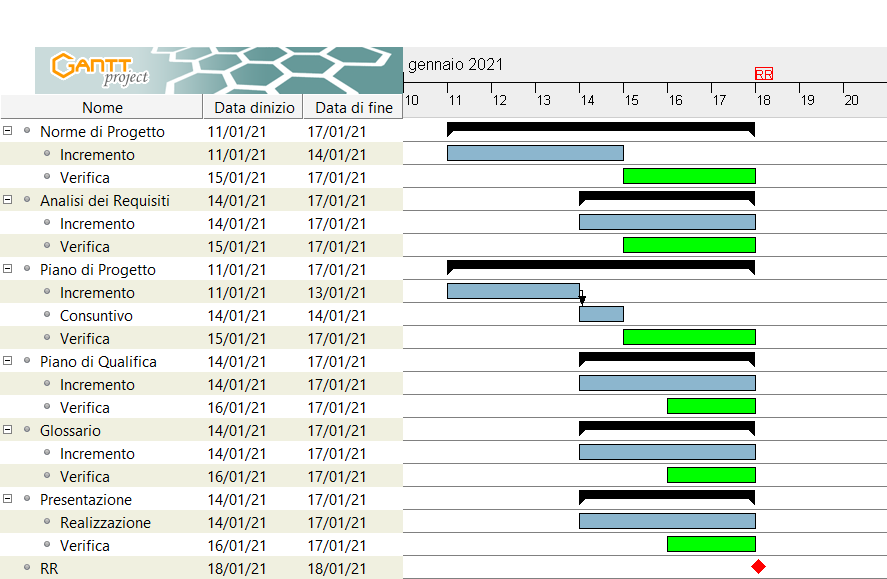
\includegraphics[width=\textwidth]{Immagini/GanttConsolidamentoRequisiti}
    \caption{Diagramma di Gantt dell'attività di consolidamento dei requisiti}
\end{figure}